% -*- LaTeX -*-
% -*- coding: utf-8 -*-
%
% ~~~~~~~~~~~~~~~~~~~~~~~~~~~~~~~~~~~~~~~~~~~~~~~~~~~~~~~~~~~~~~~~~~~~~~~~~~~~~~
%
%                             michael a.g. aïvázis
%                      california institute of technology
%                      (c) 1998-2010  all rights reserved
%
% ~~~~~~~~~~~~~~~~~~~~~~~~~~~~~~~~~~~~~~~~~~~~~~~~~~~~~~~~~~~~~~~~~~~~~~~~~~~~~~
%

\lecture{Programming with MPI}{20100125}

% --------------------------------------
% template
\begin{frame}[fragile]
%
  \frametitle{Distributed memory parallelism}
%
  \begin{itemize}
%
  \item recall the generic layout of a distributed memory machine
%
    \begin{figure}
      \centering
      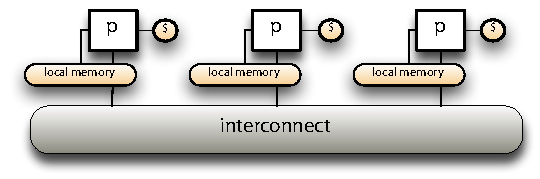
\includegraphics[scale=1.0]{figures/distributed-memory.pdf}
    \end{figure}
    \vspace{-1.0em}
%
    \begin{itemize}
      \item each processor has its own private memory space
      \item processors communicate via the interconnect substrate
    \end{itemize}
%
  \item the programming model
    \begin{itemize}
    \item program consists of a collection of $p$ named processes
      \item each process has its own instruction stream and address space
    \item logically shared data must be partitioned among the processors
    \item communication and synchronization must be orchestrated explicitly 
    \item processes communicate via explicit data exchanges
    \end{itemize}
%
  \end{itemize}
%
\end{frame}

% --------------------------------------
% template
\begin{frame}[fragile]
%
  \frametitle{\mpi\ -- the survivor}
%
  \begin{itemize}
%
  \item the {\em de facto} standard for writing parallel programs using message passing
    \begin{itemize}
    \item a library of routines callable from almost any programming language
    \item that enables communication among multiple processes
    \item standardized and portable API with good implementations available for almost any kind
      of parallel computer
    \end{itemize}
%
  \item \mpi\ is large and complex
    \begin{itemize}
    \item more than 125 functions, lot's of options and communication protocols
    \item but for most practical purposes, a small subset will suffice
    \item short introduction today, more when we consider specific physics
    \end{itemize}
%
  \item two major versions available -- check your installation for compliance
    \begin{itemize}
    \item \mpi-1: parallel machine management, process groups, collective operations,
      point-to-point operations, virtual topologies, profiling
    \item \mpi-2: dynamic process management, one-sided operations, parallel I/O, (simplistic)
      bindings for \cpp
    \end{itemize}
%
  \item \identifier{openmpi}: currently the best open source implementation
    \begin{itemize}
    \item well-architected, thread safe, fast, decent support from a broad community
    \end{itemize}
  \end{itemize}
%
\end{frame}

% --------------------------------------
% compiling, linking, staging and launching
\begin{frame}[fragile]
%
  \frametitle{Getting started}
%
  \begin{itemize}
%
  \item compiling and linking:
    \begin{itemize}
    \item most \mpi\ implementation supply wrappers around the available compilers
      \begin{itemize}
      \item e.g.~\identifier{mpicc}, \identifier{mpic++}, \identifier{mpif77},
        \identifier{mpif90}
      \end{itemize}
    \item it's not magic, so you can do it on your own to
      \begin{itemize}
      \item override the system defaults (without upsetting the sysadmins...)
      \item build multiple versions so you can benchmark
      \end{itemize}
    \end{itemize}
%
  \item staging and launching:
    \begin{itemize}
    \item most implementations provide \identifier{mpirun} to
      \begin{itemize}
      \item control the total number of desired processes
      \item specify the hostnames of the machines to use
      \item specify the mapping of processes to machines/CPUs/cores
      \item establish the current working directory, if possible, for all processes
      \item launch the program
      \end{itemize}
%
    \item but most installations do not permit its use; they have queuing systems instead
      \begin{itemize}
      \item \identifier{PBS}, \identifier{LSF}, \identifier{torque}, \identifier{maui}, ...
      \item specified and documented in the ``welcome'' package of most supercomputer centers
      \item scheduling of jobs, guarantee exclusive access to your allocated machines,
        establish upper time limit, charge the right account for your uses
      \end{itemize}
    \end{itemize}
%
  \end{itemize}
%
\end{frame}

% --------------------------------------
% initializing the runtime environment
\begin{frame}[fragile]
%
  \frametitle{At runtime}
%
  \begin{itemize}
%
%
  \item initializing the co\"operating processes:
    \begin{C}
int MPI_Init(int* argc, char ***argv);
    \end{C}
    \begin{itemize}
    \item note the strange signature; see \slideref{hello-world-mpi} for an example of its use
    \item some implementations -- notably \identifier{MPICH}, the reference implementation --
      used command line arguments to pass information from \identifier{mpirun} to the runtime
      environment
    \item so they need {\em write} access to the command line arguments to strip the extras
    \item thankfully, not done any more
    \end{itemize}
%
  \item must be the first \mpi\ in your program; nothing is initialized correctly until it
    returns
    \begin{itemize}
    \item if this call does not return \identifier{MPI\_SUCCESS}, you should abort
    \end{itemize}
% 
  \item don't forget to shut everything down:
    \begin{C}
int MPI_Finalize(void);
    \end{C}
%
  \item must be the last \mpi\ call in your program; nothing is in usable state after it
    returns
%
  \end{itemize}
%
\end{frame}

% --------------------------------------
% communicators
\begin{frame}[fragile]
%
  \frametitle{Groups and communicators}
%
  \begin{itemize}
%
  \item every \mpi\ process belongs to at least one {\em group}
%
  \item groups have associated {\em communicators} that provide the context for data exchanges and
      synchronization among processes
%
  \item processes in a given communicator get {\em ranked}
    \begin{itemize}
    \item a communicator of $p$ processes assigns ranks 0 through $p-1$
    \item a process can discover the communicator size and its own rank by using
      \begin{C}
int MPI_Comm_size(MPI_Comm communicator, int* size);
int MPI_Comm_rank(MPI_Comm communicator, int* rank);
      \end{C}
    \end{itemize}
% 
  \item the \mpi\ runtime environment creates the {\em global} communicator
    \begin{itemize}
    \item known as \identifier{MPI\_COMM\_WORLD}
    \item all processes are members
    \end{itemize}
% 
  \item it is good practice to learn to manage your own
    \begin{itemize}
    \item to narrow down global operations to processor subsets
    \item to promote {\em reuse}
    \item more details later
    \end{itemize}
% 
  \end{itemize}
%
\end{frame}

% --------------------------------------
% hello world
\begin{frame}[fragile]
%
  \frametitle{Hello world}
%
  \label{slide:hello-world-mpi}
%
  \begin{C}
#include <mpi.h>
#include <stdio.h>

int main(int argc, char* argv[]) {
    int status;
    int rank, size;

    /* initialize MPI */
    status = MPI_Init(&argc, &argv);
    if (status != MPI_SUCCESS) {
        printf("error in MPI_Init; aborting...\n");
        return status;
    }

    /* all good -- get process info and display it */
    MPI_Comm_rank(MPI_COMM_WORLD, &rank);
    MPI_Comm_size(MPI_COMM_WORLD, &size);
    printf("hello from %03d/%03d!\n", rank, size);

    /* shut down MPI */
    MPI_Finalize();

    return 0;
}
  \end{C}
%
\end{frame}

% --------------------------------------
% messages
\begin{frame}[fragile]
%
  \frametitle{Messages}
%
  \begin{itemize}
%
  \item in general, data exchanges through MPI calls involve
    \begin{itemize}
    \item a communicator
      \begin{itemize}
      \item specifies which processes participate in the exchange
      \item resolves process ranks into processes
      \end{itemize}        
    \item {\em collective} operations involve the entire communicator
    \item {\em point-to-point} operations require the rank of the message source or destination
    \item the details of the message payload
      \begin{itemize}
      \item the address of the source buffer
      \item the data type of the buffer contents
      \item the number of items in the buffer
      \end{itemize}
    \end{itemize}
%
    \item \mpi\ provides some data abstractions to
      \begin{itemize}
      \item hide machine dependencies in the data representations to enhance portability and
        support heterogeneous clusters
      \item support user defined data types
      \item support non-contiguous data layouts
      \end{itemize}        
      
%
  \end{itemize}
%
\end{frame}

% --------------------------------------
% global operations
\begin{frame}[fragile]
%
  \frametitle{Collective operations: global reductions}
%
  \begin{itemize}
%
  \item {\em collective} operations involve all processes in a given communicator
%
  \item the \mpi\ version of our global reduction example uses
    \begin{C}
int MPI_Allreduce(
        void* send_buffer, void* recv_buffer,
        int count, MPI_Datatype datatype, MPI_Op operation,
        MPI_Comm communicator
        );
   \end{C}
%
  \item example legal values for \identifier{MPI\_Datatype}
    \begin{itemize}
    \item \cc: \identifier{MPI\_INT}, \identifier{MPI\_LONG}, \identifier{MPI\_DOUBLE} 
    \item \fortran: \identifier{MPI\_INTEGER}, \identifier{MPI\_DOUBLE\_PRECISION},
      \identifier{MPI\_COMPLEX}
    \end{itemize}
%
  \item legal values for \identifier{MPI\_Op}
    \begin{itemize}
    \item \identifier{MPI\_MAX}, \identifier{MPI\_MIN}, \identifier{MPI\_MAXLOC},
      \identifier{MPI\_MINLOC}
    \item \identifier{MPI\_SUM}, \identifier{MPI\_PROD}
    \item \identifier{MPI\_LAND}, \identifier{MPI\_LOR}, \identifier{MPI\_LXOR}
    \item \identifier{MPI\_BAND}, \identifier{MPI\_BOR}, \identifier{MPI\_BXOR}
    \item \identifier{MPI\_REPLACE}
    \end{itemize}
%
  \end{itemize}
%
\end{frame}

% --------------------------------------
% example reduction with mpi
\begin{frame}[fragile]
%
  \frametitle{Example reduction using \mpi}
%
  \label{slide:squares-mpi}
%
  \begin{C}[basicstyle=\tt\bfseries\tiny]
#include <mpi.h>
#include <stdio.h>

int main(int argc, char* argv[]) {
    int status;
    int rank;
    int square, sum;

    /* initialize MPI */
    status = MPI_Init(&argc, &argv);
    if (status != MPI_SUCCESS) {
        printf("error in MPI_Init; aborting...\n");
        return status;
    }

    /* get the process rank */
    MPI_Comm_rank(MPI_COMM_WORLD, &rank);
    /* form the square */
    square = rank*rank;
    /* each process contributes the square of its rank */
    MPI_Allreduce(&square, &sum, 1, MPI_INT,  MPI_SUM, MPI_COMM_WORLD);
    /* print out the result */
    printf("%03d: sum = %d\n", rank, sum);

    /* shut down MPI */
    MPI_Finalize();

    return 0;
}
  \end{C}
%
\end{frame}
% end of file 
